\documentclass[]{llncs} 
\usepackage{amsmath}
\usepackage{verbatim}
\usepackage{datatool}
\usepackage{tikz}
\usetikzlibrary{arrows,shapes}
\usepackage{graphics}


\newcommand{\todo}[1]{ {\color{red}{#1} }}
\newcommand{\AtMostSeqCard}{AtMostSeqCard }


\author{Valentin Mayer-Eichberger and Toby Walsh}

\institute{NICTA and University of New South Wales \\
Locked Bag 6016, Sydney NSW 1466, Australia 
\email{\{valentin.mayer-eichberger,toby.walsh\}@nicta.com.au}
}

\title{SAT Encodings for the Car Sequencing Problem}

\begin{document} 

\maketitle

\begin{abstract} 
    Car sequencing is a well known NP-complete problem. This paper introduces encodings of this problem into CNF based
    on sequential counters. We demonstrate that SAT solvers are powerful in this domain and report new lower bounds for
    the benchmark set in the CSPlib.
\end{abstract}

\section{Introduction}

Car sequencing is the first benchmark in the constraint programming library (prob001 in CSPLib \cite{Gent99}). The
associated decision problem (is there a production sequence for cars on the assembly line satisfying the sliding
capacity constraints?) has been shown to be NP-complete.  To date, however, it has not received much attention from the
SAT community.  This is disappointing as we show here that SAT is a very effective technology to solve such problems. We
introduce several CNF encodings for this problem that demonstrate the strength of SAT solvers. Furthermore, we identify
new lower bounds by a preprocessing technique and by SAT solving.

The paper is organised as follows. First we formally introduce the car sequencing problem. Then in Section
\ref{sec:modelling} we define the CNF encodings and discuss their properties. A direct method to compute lower bounds is
explained in Section \ref{sec:lower}. In the experimental evaluation in Section \ref{sec:experiments} we compare the CNF
encodings and show results on the lower bounds. 

%\subsection{SAT Solving}
%
%First we will state some preliminary definitions and then give a brief background on satisfiability solving. 
%
%Given a set of Boolean variables $X = \{x_1, x_2 \ldots x_n\}$, a literal is of the form $x_i$ or $\neg x_i$ and a
%clause is a disjunction of literals. A formula is in conjunctive normal form (CNF) if it is a conjunction of
%disjunctions of literals. The Boolean satisfiability problem (SAT) requests a satisfying assignment to a given formula
%in CNF or a proof if no such assignment exists. A clause with one literal is called a unit clause. 
%
%The SAT problem is considered the canonical NP-complete problem, and in addition to its theoretical relevance it is used
%to solve practical problems. The general idea is to reduce a given NP-complete problem to a (possibly large) formula in
%CNF and apply a general purpose SAT solver to find an assignment or prove unsatisfiability. 
%
%In the last two decades there has been tremendous research in both theoretical and practical SAT solving techniques, for
%a comprehensive overview we refer to \cite{Biere09}. For the scope of this paper briefly we mention the basic underlying
%algorithm to most successful SAT solvers and its mayor extensions. The DPLL algorithm (\cite{Putnam60}) is a backtrack
%search that extends partial assignments and reasons in each node with a method called unit propagation (UP). UP
%identifies literals in clauses that have become unit under the current assignment and forces the assignment of this
%literal such that the clause is satisfied. Further improvements to the DPLL algorithms go under the name of
%Conflict-Driven Clause Learning (CDCL) solvers. These solvers record an appropriate reason for each conflict in the
%search and potentially prune unseen parts of the search tree. Furthermore, SAT solvers contain robust domain-independent
%branching, decision and restart heuristics and in many cases solve formulas with millions of variables and clauses. Nowadays
%application of SAT solving techniques reach from formal verification to the domain of logistical problems. 

\subsection{Car Sequencing}

Car sequencing deals with the problem of scheduling cars along an assembly line with capacity constraints for different
stations (e.g. radio, sun roof, air-conditioning, etc). Cars are partitioned into classes according to their
requirements. Let $C$ and $O$ be disjoint sets of classes and options. To each class $k\in C$ there is given a demand of
cars $d_k$ to be scheduled. Each option $l\in O$ is limited to $u_l$ occurrences on each subsequence of length $q_l$
(denoted as a capacity constraint $u_l/q_l$), i.e.  no more than $u_l$ cars with option $l$ can be sequenced among $q_l$
consecutive cars. To each class $k\in C$ we denote the set $O_k$ of options it requires and for convenience to each
option $l\in O$ we denote $C_l$ the set of classes that require this options. A solution is a valid sequence of all
cars. 

Let $n$ be the length of the total sequence. The following pseudo Boolean model is a basis for our translation to CNF.
We use 0/1 variables $x^m_i$ to denote that an object(class or option) $m$ is at position $i$. For the sequence it must
hold: 

\begin{itemize}
    \item Demand constraints: $\forall k \in C$ $$\sum^n_1 x^k_i = d_k$$                       
    \item Capacity constraints: $\forall l \in O$ with ratio $u_l/q_l$ $$\bigwedge_{i=0}^{n-q_l}(\sum_{j=1}^{q_lo} x^l_{i+j} \leq u_l )$$
\end{itemize}
        And in all positions $i \in \{1\ldots n\}$ of the sequence it must hold:                                                    
\begin{itemize}
    \item Link between classes and options: for each $k\in C$ and 
 $$\forall l \in O_k :\;\; x^k_i - x^l_i \leq 0$$  
 $$\forall l \not \in O_k : :\;\; x^k_i + x^l_i \leq 1$$  
    \item Exactly one car:  $$\sum_{k\in C} x^k_i = 1$$  
\end{itemize}

\begin{example} 
    Given classes $C = \{1,2,3\}$ and options $O = \{a,b\}$. The demands (number of cars) for the classes are $3,2,2$
    and capacity constraints on options are $1/2$ and $1/5$, respectively. Class 1 has no restrictions, class 2 requires
    option $a$ and class 3 needs options $\{a, b\}$. The only legal sequence for this problem is $[3,1,2,1,2,1,3]$,
    since class 2 and 3 cannot be sequenced after another and class 3 need to be at least 5 positions apart.
\end{example}                                     

Car sequencing in the CSPlib contains a selection of benchmark problems of this form ranging from 100 to 400 cars. Over
the years different approaches have been used to solve these instances, among them constraint programming, local search
and integer programming \cite{Regin97}\cite{Gottlieb03}\cite{Gravel05}\cite{Estellon06}\cite{Siala12}.

Car sequencing has also been treated as an optimisation problem, although the literature does not agree on a common
optimisation function and several versions have been proposed. There are several variations for the optimisation
function minimising the number of violated capacity constraints.  However, in this paper we use the definition of
\cite{Perron04}. Fortuitously for us, this transforms easily to a decision problem and SAT solving can be directly
applied.  An unsatisfiable car sequencing problem can be made solvable by adding empty slots (also called dummy cars) to
the sequence. The task is then to minimise the number of dummy cars needed for a valid sequence. A lower bound of $lb$
to an instance is shown by proving unsatisfiability with $lb-1$ dummy cars.

\section{Modelling the Car Sequencing Problem}
\label{sec:modelling}

In this section we introduce different ways to model the car sequencing problem in CNF. The basic building blocks are
cardinality constraints of the form $\sum_{i\in \{1\ldots n\}} x_{i} = d$ and $ \sum_{i\in \{1\ldots n\}} x_{i} \leq d
$.

First we will show how to translate cardinality constraints by a variant of the sequential counter encoding proposed by
\cite{Sinz05}. This can be used to model the demand and the capacity constraints. Then we show how to enforce a global
view by integrating capacity constraint into the sequential counter. 

\subsection{Sequential Counter Encoding}

We will show how to encode a cardinality constraint of the form $ \sum_{i\in \{1\ldots n\}} x_{i} = d $ where $x_i$ are
Boolean variables and $d$ is a fixed demand. The key idea is to introduce auxiliary variables to represent cumulative
sums.

In this section we use two types of variables, for each position $i$

\begin{itemize}
    \item  $x_i$ is true iff an object (class or option) is at position $i$
    \item  $s_{i,j}$ is true iff in the positions $0,1 \ldots i$ the object exists at least $j$ times (for technical
        reasons $0 \leq j \leq d+1$). 
\end{itemize} 

The following set of clauses (\ref{eq:1}) to (\ref{eq:5}) define the sequential counter encoding (SC):

$\forall i \in \{1\ldots n\}$ $\forall j \in\{0 \ldots d+1\}$: 
\begin{equation} \label{eq:1}
    \neg s_{i-1,j} \vee s_{i,j}
\end{equation}
\begin{equation} \label{eq:2}
    x_{i} \vee \neg s_{i,j} \vee s_{i-1,j}
\end{equation}

$\forall {i \in \{1\ldots n\}} \forall {j\in \{1\ldots d+1\}}$: 
\begin{equation} \label{eq:3}
    \neg s_{i,j} \vee s_{i-1,j-1}
\end{equation}
\begin{equation} \label{eq:4}
    \neg x_{i} \vee \neg s_{i-1,j-1} \vee s_{i,j}
\end{equation}
\begin{equation} \label{eq:5}
     s_{0,0} \wedge \neg s_{0,1} \wedge s_{n,d} \wedge \neg s_{n,d+1}
\end{equation}

%\begin{proposition}
%Under any partial assignment on the variables of the SC encoding, UP forces  all entailed values. 
%\end{proposition}

The variables $s_{i,j}$  represent the bounds for cumulative sums for the sequence $x_1 \ldots x_i$. The encoding is
best explained by visualising $s_{i,j}$ as a two dimensional grid with positions (horisontal) and cumulative sums
(vertical). The binary clauses (\ref{eq:1}) and (\ref{eq:3}) ensures that the counter (i.e. the variables representing
the cumulative sums) is monotonically increasing. Clauses (\ref{eq:2}) and (\ref{eq:4}) control the interaction with the
variables $x_i$. If $x_i$ is true, then the counter has to increase at position $i$ whereas if $x_i$ is false an
increase is prevented at position $i$. The conjunction (\ref{eq:5}) sets the initial values for the counter to start
counting at 0 and ensures that the total sum at position $n$ is equal to $d$. 


\begin{example}
The auxiliary variables $s_{i,j}$ with $d=2$ over a sequence of 10 variables. The cells with  $U$($L$) and
above(below) are set to false (true) by preprocessing. The question mark identifies yet unassigned variables. Left:
before variable assignments, right: after variable assignment $x_2$ and $x_7$ to true.
\begin{center}
\begin{minipage}[t]{0.5\textwidth}
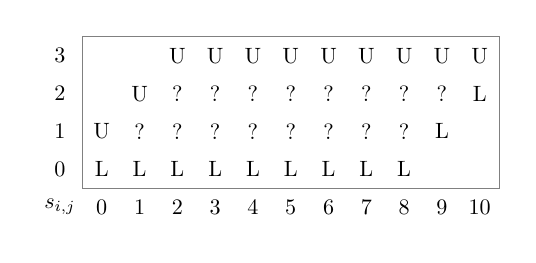
\begin{tikzpicture}[scale=0.8,every node/.style={scale=0.8}]
\node [matrix,ampersand replacement=\&,nodes={minimum size=6mm}]
%,nodes={fill=blue!20,minimum size=5mm}] 
    {
        \node {3}; \& \node (x) { }; \& \node { }; \& \node {U}; \& \node {U}; \& \node {U}; \& \node {U}; \& \node {U}; \& \node {U}; \& \node {U}; \& \node {U}; \& \node {U}; \\
        \node {2}; \& \node { }; \& \node {U}; \& \node {?}; \& \node {?}; \& \node {?}; \& \node {?}; \& \node {?}; \& \node {?}; \& \node {?}; \& \node {?}; \& \node {L}; \\
        \node {1}; \& \node {U}; \& \node {?}; \& \node {?}; \& \node {?}; \& \node {?}; \& \node {?}; \& \node {?}; \& \node {?}; \& \node {?}; \& \node {L}; \& \node { }; \\
        \node {0}; \& \node {L}; \& \node {L}; \& \node {L}; \& \node {L}; \& \node {L}; \& \node {L}; \& \node {L}; \& \node {L}; \& \node {L}; \& \node { }; \& \node (y) { }; \\
        \node {$s_{i,j}$}; \& \node {0}; \& \node {1}; \& \node {2}; \& \node {3}; \& \node {4}; \& \node {5}; \& \node {6}; \& \node {7}; \& \node {8}; \& \node {9}; \& \node {10}; \\
};
\draw[gray] (x.north west) rectangle (y.south east);
\end{tikzpicture}


\end{minipage}%
\begin{minipage}[t]{0.5\textwidth}
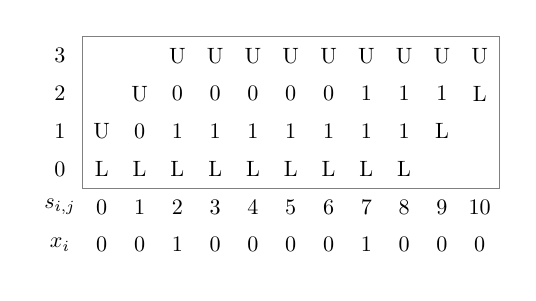
\begin{tikzpicture}[scale=0.8,every node/.style={scale=0.8}]    
\node [matrix,ampersand replacement=\&,nodes={minimum size=6mm}]
%,nodes={fill=blue!20,minimum size=5mm}] 
    {
        \node {3}; \& \node (x) { }; \& \node { }; \& \node {U}; \& \node {U}; \& \node {U}; \& \node {U}; \& \node {U}; \& \node {U}; \& \node {U}; \& \node {U}; \& \node {U}; \\
        \node {2}; \& \node { }; \& \node {U}; \& \node {0}; \& \node {0}; \& \node {0}; \& \node {0}; \& \node {0}; \& \node {1}; \& \node {1}; \& \node {1}; \& \node {L}; \\
        \node {1}; \& \node {U}; \& \node {0}; \& \node {1}; \& \node {1}; \& \node {1}; \& \node {1}; \& \node {1}; \& \node {1}; \& \node {1}; \& \node {L}; \& \node { }; \\
        \node {0}; \& \node {L}; \& \node {L}; \& \node {L}; \& \node {L}; \& \node {L}; \& \node {L}; \& \node {L}; \& \node {L}; \& \node {L}; \& \node { }; \& \node (y) { }; \\
        \node {$s_{i,j}$}; \& \node {0}; \& \node {1}; \& \node {2}; \& \node {3}; \& \node {4}; \& \node {5}; \& \node {6}; \& \node {7}; \& \node {8}; \& \node {9}; \& \node {10}; \\
        \node {$x_{i}$}; \& \node {0}; \& \node {0}; \& \node {1}; \& \node {0}; \& \node {0}; \& \node {0}; \& \node {0}; \& \node {1}; \& \node {0}; \& \node {0}; \& \node {0}; \\
};
\draw[gray] (x.north west) rectangle (y.south east);
\end{tikzpicture}


\end{minipage}
\end{center}
\label{ex:1}
\end{example}

The encoding in \cite{Sinz05} follows a similar idea and focuses on $\leq$ expressions. SC can be adapted to represent
such constraints by removing $s_{n,d}$ from the conjunction (\ref{eq:5}). Then the counter accepts all assignments to
$x_1 \ldots x_n$ with up to $d$ variables set to true. Comparing the resulting clauses there are certain differences
between the encoding proposed here and the one in \cite{Sinz05}. We post twice as many clauses and ensure uniqueness by
the auxiliary variables, i.e. we ensure the same model count. 

\subsection{The Capacity Constraint}

We now show how to translate the interleaving capacity constraints to CNF. Each subsequence of length $q$ can have at
most $u$ true assignments. Thus, the capacity constraints are a sequence of cardinality expressions. 

$$\bigwedge_{i=0}^{n-q}(\sum_{l=1}^q x_{i+l} \leq u )$$

We will translate this expression to CNF in two ways. The straight forward way is to encode a sequential counter for
each subsequence separately. This will introduce independent auxiliary variables for each subsequence. The second way is
more elaborate and is explained in this section.

The idea is to encode a more global view into the demand constraint by integrating the capacity of each subsequence into
the counter. We intend to encode the global view on the following expression: 

$$ (\sum_{i=1}^n x_{i} = d) \wedge \bigwedge_{i=0}^{n-q}(\sum_{l=1}^q x_{i+l} \leq u )$$

Interestingly, we can reuse the auxiliary variables of the SC encoding and impose the following set of clauses: 

$\forall {i \in \{q \ldots n\}}$, $\forall {j\in\{u\ldots d+1\}}$: 

\begin{equation} \label{eq:6}
    \neg s_{i,j} \vee s_{i-q,j-u}
\end{equation}               

The clauses restrict the internal counting not to exceed the capacities constraints. The following example will demonstrate
the way these clauses work. 

\begin{example}
\label{ex:large} See tables in Figure \ref{fig3} for a visualisation of the variables. We construct the grid for a
capacity constraint $4/8$ and a demand of $d=12$ on a sequence of 22 variables. UP will force $x_{7}$, $x_{8}$, $x_{15}$
and $x_{16}$ to be false prior to search. The second table examines the variables after decisions $x_{1}$ and $x_{13}$ to
true and $x_{12}$, $x_{14}$ and $x_{21}$ to false. Notice the amount of propagation due to the clauses (\ref{eq:6}), the
interesting two cases are shown by an arrow. (Configuration of this example taken from  \cite{Siala12}). 
\end{example}

\begin{figure}
\centering 
\caption{The grid of variables of Example \ref{ex:large}. Notation for bottom row: normal font = decision variable, bold
= propagated, in brackets = propagated previously.}
\begin{tikzpicture}
\node [matrix,ampersand replacement=\&,nodes={minimum size=6mm}]
%,nodes={fill=blue!20,minimum size=5mm}] 
    {
\node{13}; \& \node (x) { }; \& \node { }; \& \node { }; \& \node { }; \& \node { }; \& \node { }; \& \node { }; \& \node { }; \& \node { }; \& \node { }; \& \node { }; \& \node { }; \& \node { }; \& \node { }; \& \node { }; \& \node { }; \& \node { }; \& \node { }; \& \node { }; \& \node { }; \& \node {U}; \& \node {U}; \& \node {U}; \\
\node{12}; \& \node { }; \& \node { }; \& \node { }; \& \node { }; \& \node { }; \& \node { }; \& \node { }; \& \node { }; \& \node { }; \& \node { }; \& \node { }; \& \node { }; \& \node { }; \& \node { }; \& \node { }; \& \node { }; \& \node { }; \& \node { }; \& \node { }; \& \node {U}; \& \node {?}; \& \node {?}; \& \node {L}; \\
\node{11}; \& \node { }; \& \node { }; \& \node { }; \& \node { }; \& \node { }; \& \node { }; \& \node { }; \& \node { }; \& \node { }; \& \node { }; \& \node { }; \& \node { }; \& \node { }; \& \node { }; \& \node { }; \& \node { }; \& \node { }; \& \node { }; \& \node {U}; \& \node {?}; \& \node {?}; \& \node {L}; \& \node { }; \\
\node{10}; \& \node { }; \& \node { }; \& \node { }; \& \node { }; \& \node { }; \& \node { }; \& \node { }; \& \node { }; \& \node { }; \& \node { }; \& \node { }; \& \node { }; \& \node { }; \& \node { }; \& \node { }; \& \node { }; \& \node { }; \& \node {U}; \& \node {?}; \& \node {?}; \& \node {L}; \& \node { }; \& \node { }; \\
\node{9}; \& \node { }; \& \node { }; \& \node { }; \& \node { }; \& \node { }; \& \node { }; \& \node { }; \& \node { }; \& \node { }; \& \node { }; \& \node { }; \& \node { }; \& \node {U}; \& \node {U}; \& \node {U}; \& \node {U}; \& \node {U}; \& \node {?}; \& \node {?}; \& \node {L}; \& \node { }; \& \node { }; \& \node { }; \\
\node{8}; \& \node { }; \& \node { }; \& \node { }; \& \node { }; \& \node { }; \& \node { }; \& \node { }; \& \node { }; \& \node { }; \& \node { }; \& \node { }; \& \node {U}; \& \node {?}; \& \node {?}; \& \node {L}; \& \node {L}; \& \node {L}; \& \node {L}; \& \node {L}; \& \node { }; \& \node { }; \& \node { }; \& \node { }; \\
\node{7}; \& \node { }; \& \node { }; \& \node { }; \& \node { }; \& \node { }; \& \node { }; \& \node { }; \& \node { }; \& \node { }; \& \node { }; \& \node {U}; \& \node {?}; \& \node {?}; \& \node {L}; \& \node { }; \& \node { }; \& \node { }; \& \node { }; \& \node { }; \& \node { }; \& \node { }; \& \node { }; \& \node { }; \\
\node{6}; \& \node { }; \& \node { }; \& \node { }; \& \node { }; \& \node { }; \& \node { }; \& \node { }; \& \node { }; \& \node { }; \& \node {U}; \& \node {?}; \& \node {?}; \& \node {L}; \& \node { }; \& \node { }; \& \node { }; \& \node { }; \& \node { }; \& \node { }; \& \node { }; \& \node { }; \& \node { }; \& \node { }; \\
\node{5}; \& \node { }; \& \node { }; \& \node { }; \& \node { }; \& \node {U}; \& \node {U}; \& \node {U}; \& \node {U}; \& \node {U}; \& \node {?}; \& \node {?}; \& \node {L}; \& \node { }; \& \node { }; \& \node { }; \& \node { }; \& \node { }; \& \node { }; \& \node { }; \& \node { }; \& \node { }; \& \node { }; \& \node { }; \\
\node{4}; \& \node { }; \& \node { }; \& \node { }; \& \node {U}; \& \node {?}; \& \node {?}; \& \node {L}; \& \node {L}; \& \node {L}; \& \node {L}; \& \node {L}; \& \node { }; \& \node { }; \& \node { }; \& \node { }; \& \node { }; \& \node { }; \& \node { }; \& \node { }; \& \node { }; \& \node { }; \& \node { }; \& \node { }; \\
\node{3}; \& \node { }; \& \node { }; \& \node {U}; \& \node {?}; \& \node {?}; \& \node {L}; \& \node { }; \& \node { }; \& \node { }; \& \node { }; \& \node { }; \& \node { }; \& \node { }; \& \node { }; \& \node { }; \& \node { }; \& \node { }; \& \node { }; \& \node { }; \& \node { }; \& \node { }; \& \node { }; \& \node { }; \\
\node{2}; \& \node { }; \& \node {U}; \& \node {?}; \& \node {?}; \& \node {L}; \& \node { }; \& \node { }; \& \node { }; \& \node { }; \& \node { }; \& \node { }; \& \node { }; \& \node { }; \& \node { }; \& \node { }; \& \node { }; \& \node { }; \& \node { }; \& \node { }; \& \node { }; \& \node { }; \& \node { }; \& \node { }; \\
\node{1}; \& \node {U}; \& \node {?}; \& \node {?}; \& \node {L}; \& \node { }; \& \node { }; \& \node { }; \& \node { }; \& \node { }; \& \node { }; \& \node { }; \& \node { }; \& \node { }; \& \node { }; \& \node { }; \& \node { }; \& \node { }; \& \node { }; \& \node { }; \& \node { }; \& \node { }; \& \node { }; \& \node { }; \\
\node{0}; \& \node {L}; \& \node {L}; \& \node {L}; \& \node { }; \& \node { }; \& \node { }; \& \node { }; \& \node { }; \& \node { }; \& \node { }; \& \node { }; \& \node { }; \& \node { }; \& \node { }; \& \node { }; \& \node { }; \& \node { }; \& \node { }; \& \node { }; \& \node { }; \& \node { }; \& \node { }; \& \node (y) { }; \\
\node{j/i}; \& \node {0}; \& \node {1}; \& \node {2}; \& \node {3}; \& \node {4}; \& \node {5}; \& \node {6}; \& \node {7}; \& \node {8}; \& \node {9}; \& \node {10}; \& \node {11}; \& \node {12}; \& \node {13}; \& \node {14}; \& \node {15}; \& \node {16}; \& \node {17}; \& \node {18}; \& \node {19}; \& \node {20}; \& \node {21}; \& \node {22}; \\
\node{$x_i$}; \& \node { }; \& \node { }; \& \node { }; \& \node { }; \&
        \node { }; \& \node { }; \& \node { }; \& \node {\textbf{0}}; \&
        \node {\textbf{0}}; \& \node { }; \& \node { }; \& \node { }; \&
        \node { }; \& \node { }; \& \node { }; \& \node {\textbf{0}}; \&
        \node {\textbf{0}}; \& \node { }; \& \node { }; \& \node { }; \& \node { }; \& \node { }; \& \node { }; \\
};
\draw[gray] (x.north west) rectangle (y.south east);
\end{tikzpicture}


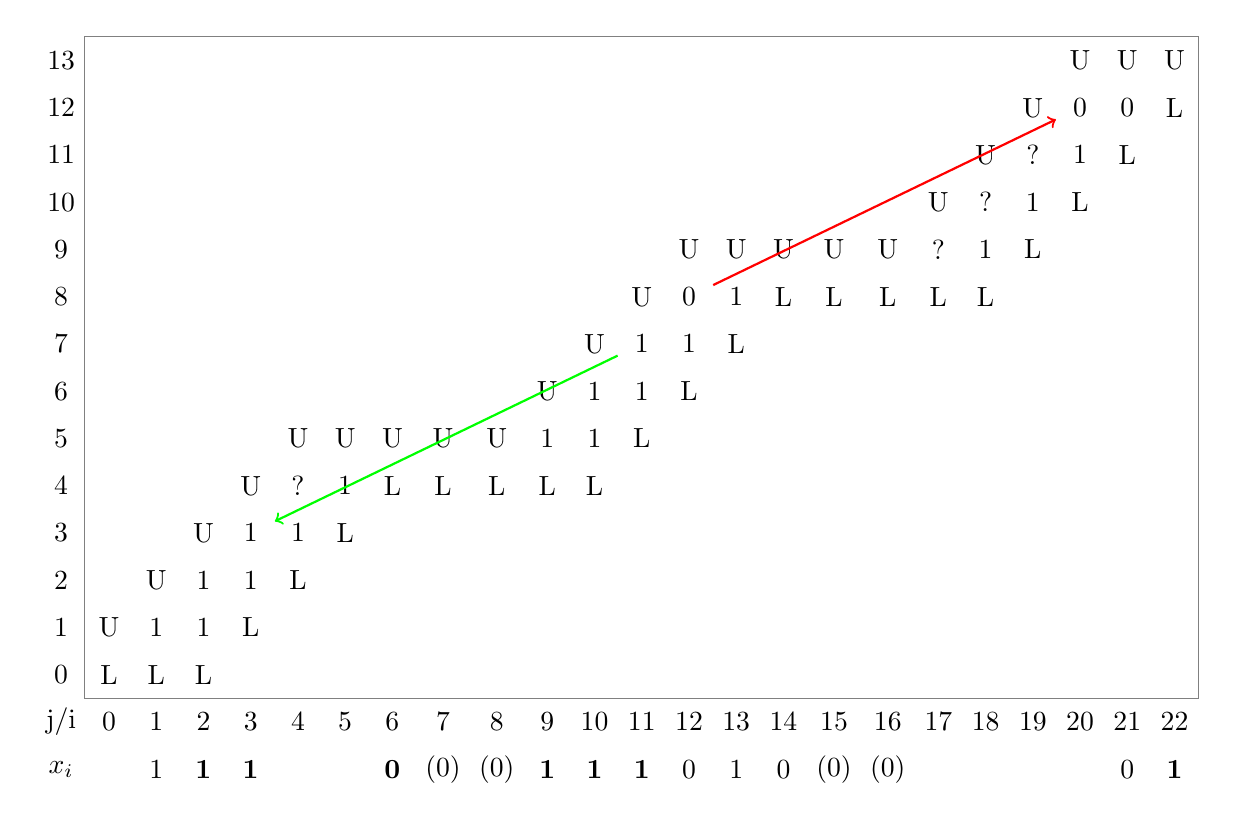
\begin{tikzpicture}
\node [matrix,ampersand replacement=\&,nodes={minimum size=6mm}]
    {
\node {13}; \& \node (x) { }; \& \node { }; \& \node { }; \& \node { }; \& \node { }; \& \node { }; \& \node { }; \& \node { }; \& \node { }; \& \node { }; \& \node { }; \& \node { }; \& \node { }; \& \node { }; \& \node { }; \& \node { }; \& \node { }; \& \node { }; \& \node { }; \& \node { }; \& \node {U}; \& \node {U}; \& \node {U}; \\
\node {12}; \& \node { }; \& \node { }; \& \node { }; \& \node { }; \&
        \node { }; \& \node { }; \& \node { }; \& \node { }; \& \node {
    }; \& \node { }; \& \node { }; \& \node { }; \& \node { }; \& \node
        { }; \& \node { }; \& \node { }; \& \node { }; \& \node { }; \&
        \node { }; \& \node {U}; \& \node (b) {0}; \& \node {0}; \& \node {L}; \\
\node {11}; \& \node { }; \& \node { }; \& \node { }; \& \node { }; \& \node { }; \& \node { }; \& \node { }; \& \node { }; \& \node { }; \& \node { }; \& \node { }; \& \node { }; \& \node { }; \& \node { }; \& \node { }; \& \node { }; \& \node { }; \& \node { }; \& \node {U}; \& \node {?}; \& \node {1}; \& \node {L}; \& \node { }; \\
\node {10}; \& \node { }; \& \node { }; \& \node { }; \& \node { }; \& \node { }; \& \node { }; \& \node { }; \& \node { }; \& \node { }; \& \node { }; \& \node { }; \& \node { }; \& \node { }; \& \node { }; \& \node { }; \& \node { }; \& \node { }; \& \node {U}; \& \node {?}; \& \node {1}; \& \node {L}; \& \node { }; \& \node { }; \\
\node {9}; \& \node { }; \& \node { }; \& \node { }; \& \node { }; \& \node { }; \& \node { }; \& \node { }; \& \node { }; \& \node { }; \& \node { }; \& \node { }; \& \node { }; \& \node {U}; \& \node {U}; \& \node {U}; \& \node {U}; \& \node {U}; \& \node {?}; \& \node {1}; \& \node {L}; \& \node { }; \& \node { }; \& \node { }; \\
\node {8}; \& \node { }; \& \node { }; \& \node { }; \& \node { }; \& \node { }; \& \node { }; \& \node { }; \& \node { }; \& \node { }; \& \node { }; \& \node { }; \& \node {U}; \& \node (a) {0}; \& \node {1}; \& \node {L}; \& \node {L}; \& \node {L}; \& \node {L}; \& \node {L}; \& \node { }; \& \node { }; \& \node { }; \& \node { }; \\
\node {7}; \& \node { }; \& \node { }; \& \node { }; \& \node { }; \&
        \node { }; \& \node { }; \& \node { }; \& \node { }; \& \node {
    }; \& \node { }; \& \node {U}; \& \node (c) {1}; \& \node {1}; \& \node {L}; \& \node { }; \& \node { }; \& \node { }; \& \node { }; \& \node { }; \& \node { }; \& \node { }; \& \node { }; \& \node { }; \\
\node {6}; \& \node { }; \& \node { }; \& \node { }; \& \node { }; \& \node { }; \& \node { }; \& \node { }; \& \node { }; \& \node { }; \& \node {U}; \& \node {1}; \& \node {1}; \& \node {L}; \& \node { }; \& \node { }; \& \node { }; \& \node { }; \& \node { }; \& \node { }; \& \node { }; \& \node { }; \& \node { }; \& \node { }; \\
\node {5}; \& \node { }; \& \node { }; \& \node { }; \& \node { }; \& \node {U}; \& \node {U}; \& \node {U}; \& \node {U}; \& \node {U}; \& \node {1}; \& \node {1}; \& \node {L}; \& \node { }; \& \node { }; \& \node { }; \& \node { }; \& \node { }; \& \node { }; \& \node { }; \& \node { }; \& \node { }; \& \node { }; \& \node { }; \\
\node {4}; \& \node { }; \& \node { }; \& \node { }; \& \node {U}; \& \node {?}; \& \node {1}; \& \node {L}; \& \node {L}; \& \node {L}; \& \node {L}; \& \node {L}; \& \node { }; \& \node { }; \& \node { }; \& \node { }; \& \node { }; \& \node { }; \& \node { }; \& \node { }; \& \node { }; \& \node { }; \& \node { }; \& \node { }; \\
        \node {3}; \& \node { }; \& \node { }; \& \node {U}; \& \node
        (d) {1}; \& \node {1}; \& \node {L}; \& \node { }; \& \node { }; \& \node { }; \& \node { }; \& \node { }; \& \node { }; \& \node { }; \& \node { }; \& \node { }; \& \node { }; \& \node { }; \& \node { }; \& \node { }; \& \node { }; \& \node { }; \& \node { }; \& \node { }; \\
\node {2}; \& \node { }; \& \node {U}; \& \node {1}; \& \node {1}; \& \node {L}; \& \node { }; \& \node { }; \& \node { }; \& \node { }; \& \node { }; \& \node { }; \& \node { }; \& \node { }; \& \node { }; \& \node { }; \& \node { }; \& \node { }; \& \node { }; \& \node { }; \& \node { }; \& \node { }; \& \node { }; \& \node { }; \\
\node {1}; \& \node {U}; \& \node {1}; \& \node {1}; \& \node {L}; \& \node { }; \& \node { }; \& \node { }; \& \node { }; \& \node { }; \& \node { }; \& \node { }; \& \node { }; \& \node { }; \& \node { }; \& \node { }; \& \node { }; \& \node { }; \& \node { }; \& \node { }; \& \node { }; \& \node { }; \& \node { }; \& \node { }; \\
\node {0}; \& \node {L}; \& \node {L}; \& \node {L}; \& \node { }; \& \node { }; \& \node { }; \& \node { }; \& \node { }; \& \node { }; \& \node { }; \& \node { }; \& \node { }; \& \node { }; \& \node { }; \& \node { }; \& \node { }; \& \node { }; \& \node { }; \& \node { }; \& \node { }; \& \node { }; \& \node { }; \& \node (y) { }; \\
\node {j/i}; \& \node {0}; \& \node {1}; \& \node {2}; \& \node {3}; \& \node {4}; \& \node {5}; \& \node {6}; \& \node {7}; \& \node {8}; \& \node {9}; \& \node {10}; \& \node {11}; \& \node {12}; \& \node {13}; \& \node {14}; \& \node {15}; \& \node {16}; \& \node {17}; \& \node {18}; \& \node {19}; \& \node {20}; \& \node {21}; \& \node {22}; \\
        \node{$x_i$}; \& \node {}; \& \node {1}; \& \node {\textbf{1}}; \& \node { \textbf{1}}; \& \node { }; \& \node { }; \& \node {\textbf{0} }; \& \node {(0)}; \& \node {(0)}; \& \node {\textbf{1} }; \& \node {\textbf{1} }; \& \node {\textbf{1} }; \& \node {0}; \& \node {1}; \& \node {0}; \& \node {(0)}; \& \node {(0)}; \& \node { }; \& \node { }; \& \node { }; \& \node { }; \& \node {0}; \& \node {\textbf{1}}; \\
};
\draw[thick,red,->, sloped, above] (a) -- (b); 
\draw[thick,green,->,bend right] (c) -- (d); 
\draw[gray] (x.north west) rectangle (y.south east);
\end{tikzpicture}       

\label{fig3}
\end{figure}

\subsection{Link Cars and Options}

For a complete CNF translation of car sequencing we need to link classes and options. This is done by the following
clauses. 

$\forall i\in \{1\ldots n\}$: 

\begin{equation} \label{eq:7}
     \bigwedge_{\substack{k \in C \\ l \in O_k }} \neg x^k_{i} \vee x^l_{i}
\end{equation}

\begin{equation} \label{eq:8}
    \bigwedge_{\substack{k \in C \\ l \not \in O_k}} \neg x^k_{i} \vee \neg x^l_{i}
\end{equation}

\begin{equation} \label{eq:9}
    \bigwedge_{l\in O} \left(\neg x^l_{i} \vee \bigvee_{k \in C_l} x^k_{i}\right)
\end{equation}

Clause (\ref{eq:7}) and (\ref{eq:8}) follow directly from the pseudo Boolean model, whereas we add (\ref{eq:9}) to
ensure more propagation when e.g. branched negatively on a set of variables of classes such that a support for an
option is lost and its variable should be false.

Furthermore, for each position an additional sequential counter is used to restrict the number of cars to exactly one. 

%However they are incomparable when it comes to UP and should be added both: 
%
%\begin{proposition}
%    UP pruning is incomparable between (\ref{eq:8}) and (\ref{eq:9}).
%\end{proposition}
%\begin{proof}
%    We show two examples: If branched positively on an option, then clause (\ref{eq:8}) triggers by UP all classes that
%    do not have this option to false. This is not detected by (\ref{eq:9}). On the other hand if branched negatively on a
%    class that has one option that no other class has, then that option is set to false by UP through clause
%    (\ref{eq:9}).
%\end{proof}

\subsection{The Complete Model}

For each class we are given a cardinality constraint by the demands and for each option a capacity rule. From this we
can identify for each option $l \in O$ its implicit demand by summing up the demand of all classes that require this options.

$$ d_l = \sum_{k\in C_l} d_k$$

Moreover, we can determine for each class the strictest capacity constraint from all its options. Thus, classes and
options are translated to CNF in a uniform way, by a demand constraint and by interleaving capacity constraints. The
link between classes and options for all models is encoded by clauses (\ref{eq:7}),(\ref{eq:8}) and (\ref{eq:9}). For
our experimental section we define three models E1, E2 and E3 that vary in the way the demand and capacity constraints
are translated. 

\begin{itemize}
    \item E1 translates demand and capacity constraints separately by the clauses (\ref{eq:1}) to (\ref{eq:5}). 
    \item E2 translates these constraints by the integrated way using clauses (\ref{eq:1}) to (\ref{eq:6}).
    \item E3 combines both E1 and E2. 
\end{itemize}

\section{Lower Bounds by Preprocessing}
\label{sec:lower}

The idea to this method goes back to the proof in \cite{Gent98} to show a lower bound of 2 for the instance 19/97. Here
we will restate this technique to apply the method on all problems from the benchmark in \cite{Gravel05}. 

We start with instance 300-04 as an example. The demands and options are given in Table \ref{tab:2}. 

\begin{table}[htbp]
    \caption{Overview of options and demands for instance 300-04}
    \centering
    %%%%%%%%%%%%%%%%%%%%%%%%%%%%%%%%%%%%%%%%%%%%%%%%%%%%%%%%%%%%%%%%%%%%%%
%%                                                                  %%
%%  This is a LaTeX2e table fragment exported from Gnumeric.        %%
%%                                                                  %%
%%%%%%%%%%%%%%%%%%%%%%%%%%%%%%%%%%%%%%%%%%%%%%%%%%%%%%%%%%%%%%%%%%%%%%
\begin{tabular*}{1\linewidth}{@{\extracolsep{\fill}} c|rrrrrrrrrrrr}
class	&0	&1	&2	&3	&4	&5	&6	&7	&8	&9	&10	&11	\\
demand	&9	&4	&22	&2	&1	&62	&31	&4	&24	&4	&3	&36	\\
  \hline                        
0: $1/2$	&-	&-	&-	&-	&-	&-	&-	&-	&-	&-	&-  &x \\
1: $2/3$	&-	&-	&-	&-	&-	&x	&x	&x	&x	&x	&x  &- \\
2: $1/3$	&-	&-	&x	&x	&x	&-	&-	&-	&x	&x	&x  &- \\
3: $2/5$	&-	&x	&-	&-	&x	&-	&x	&x	&-	&-	&x  &- \\
4: $1/5$	&x	&x	&-	&x	&x	&-	&-	&x	&-	&x	&x  &- \\
\end{tabular*}

\vspace{1cm}

\begin{tabular*}{1\linewidth}{@{\extracolsep{\fill}} c|rrrrrrrrrrrrr}
class		&12	&13	&14	&15	&16	&17	&18	&19	&20	&\textbf{21} &22 &\textbf{23}\\
demand		&3	&25	&3	&8	&5	&2	&6	&21	&5	&\textbf{7 } &11 &\textbf{2}\\
  \hline
0: $1/2$	&x	&x	&x	&x	&x	&x	&x	&x	&x	&\textbf{x } &x	 &\textbf{x}\\
1: $2/3$	&-	&-	&-	&-	&-	&-	&x	&x	&x	&\textbf{x } &x	 &\textbf{x}\\
2: $1/3$	&-	&-	&-	&x	&x	&x	&-	&-	&-	&\textbf{x } &x	 &\textbf{x}\\
3: $2/5$	&-	&x	&x	&-	&-	&x	&-	&x	&x	&\textbf{- } &x	 &\textbf{x}\\
4: $1/5$	&x	&-	&x	&-	&x	&x	&x	&-	&x	&\textbf{x } &-	 &\textbf{x}\\
\end{tabular*}

    \label{tab:2}
\end{table}

There are two classes, 21 and 23, that require options 0, 1, 2 and 4 and sum of demands is 9. First observation is that
all other classes share at least one option with these two classes.  Secondly cars of class 21 and 23 have to be put at
least 5 apart, so they cannot share a neighbour. Furthermore, they cannot be neighbour to any of the classes that have a
$1/q$ restriction. This leaves us with the classes that only share the option 1 and for each car at most one adjacent
car can have restriction $2/3$. Since the first and the last car in the sequence can have any neighbour with that
restriction, the number of cars that share no option is at least $9-2=7$. Since there are no such cars, the lower bound
for this problem is 7. 

A similar argument can be made for classes 21, 22, 23 that share options 0, 1 and 2. Here the collective demand is 20
and the supply of cars that have neither of these options is $20 - 13 = 7$. This gives a lower bound of 5, which is
weaker than the first case. 

%The general idea is to compute the demand for classes that share a subset of options such that there is a lower bound on
%the number of cars that do not share any options with this subset.

We unify the two cases into a method that can then be used to compute lower bounds. Given a set of options $B\subseteq
O$ that contain the following capacity constraint: at least one of the form $1/q$ where $q \geq 3$ and at most one with
$2/r$ where $r \geq 3$ and arbitrary many $1/s$ for $s \geq 2$. If the total demand for this set is $d_B$, then there
have to be at least $d_B-2$ cars that do not require any of these options in $B$. The reason for this is as in the
example above. Cars that have all options in $B$ are at least 3 positions apart and thus cannot share an adjacent car.
Cars that share at least one option with $B$ can at most occupy one side since the weakest restriction is $2/r$ and
consequently for a valid sequence cars that contain no option in $B$ are needed. Edge cases (start and end of the
sequence) are removed and thus we need $d_B-2$ cars with no options in $B$. A lower bound is then the difference of
demand and availability of such cars. 

%\begin{proof}
%    still working on it...
%    For convenience we describe sequences of cars by words of the alphabet $\{a,b,c\}$, $a$ denotes a car that requires
%    at least one option in $B$, $b$ denotes a car that requires all options in $B$ and $c$ denotes a car that requires
%    no option in $B$. 
%    \begin{enumerate}
%        \item For each car having all options in $B$ there cannot be cars next to it that require at least one option in
%            $B$.  Neighbours can be shared, so the sequence as $bcbcbc\ldots cb$ is one with least number of $c$s
%            necessary. Thus there have to be at least $k-1$ cars with no option of $B$. 
%        \item Similar to 1) but here neighbours cannot be shared. 
%        \item Neighbours cannot be shared and due to the capacity constraint with $2/q$ one of the neighbors. 
%    \end{enumerate}
%\end{proof}

\section{Evaluation}
\label{sec:experiments}
                                                                      
First we will compare the three different SAT encodings of Section \ref{sec:modelling} on the CSPlib instances. Then we
show our results for lower bounds. Our focus is on the 9 traditional instances plus the 30 hard instances proposed by
\cite{Gravel05}. We leave out the set of 70 easy instances, as all of them can be solved in under 2 second and the
difference among the models is minimal. 

We have written a command line tool that generates CNF in DIMACS format from a problem description as provided by the
CSPlib. It can on request translate the specification by different sets of clauses and compute the lower bounds from the
preprocessing as defined in Section \ref{sec:lower}. It is freely available at \verb+github.com/vale1410/car-sequencing+.

For our experiments we choose the well-known SAT solver Minisat \cite{Een03} of version 2.2.0, that represents a
canonical implementation of state-of-the-art CDCL solvers. All experiments are done on Linux 64bit, Intel Xeon CPUs at
2.27GHs.

\begin{table}[htbp]
    \caption{SAT solving on the three different models.}
    \centering
    \begin{minipage}[t]{0.5\textwidth}
    \begin{center}
    %%%%%%%%%%%%%%%%%%%%%%%%%%%%%%%%%%%%%%%%%%%%%%%%%%%%%%%%%%%%%%%%%%%%%%
%%                                                                  %%
%%  This is a LaTeX2e table fragment exported from Gnumeric.        %%
%%                                                                  %%
    %%%%%%%%%%%%%%%%%%%%%%%%%%%%%%%%%%%%%%%%%%%%%%%%%%%%%%%%%%%%%%%%%%%%%%
%\begin{tabular}{ lc|ccc }
%Instance &Result &E1	    &E2	    &E3 \\
%    \hline
%4/72	&SAT	&0.2	&0.2	&0.1\\
%6/76	&UNSAT	&6.5	&8.2	&18.3\\
%10/93	&UNSAT	&8.8	&17.3	&17.5\\
%16/81	&SAT	&0.3	&0.1	&0.1\\
%19/71	&-	&-	&-	&-\\
%21/90	&UNSAT	&157.9	&93.8	&288.3\\
%36/92	&UNSAT	&23.5	&54.2	&57.9\\
%41/66	&SAT	&0.0	&0.0	&0.1\\
%26/82	&SAT	&0.6	&0.1	&0.1\\
% & & & &  \\
%200-01	&SAT	&76.5	&68.1	&7.5\\
%200-02	&-	&-	&-	&-\\
%200-03	&UNSAT	&26.9	&20.5	&35.1\\
%200-04	&UNSAT	&116.2	&372.2	&15.5\\
%200-05	&UNSAT	&515.5	&-	&1381.4\\
%200-06	&-	&-	&-	&-\\
%200-07	&SAT	&8.1	&2.2	&0.8\\
%200-08	&-	&-	&-	&-\\
%200-09	&UNSAT	&192.9	&-	&-\\
%200-10	&UNSAT	&2.7	&5.7	&5.1\\
%    \hline
%\end{tabular}

\begin{tabular}{ l|ccccc }
Inst(SAT)\;\;\;\; &E1 &E2 &E3 &ASP    &PB\\
    \hline
4/72   &0.14   &0.17   &{\bf 0.05}   &6.78   &-\\
16/81  &0.38   &{\bf 0.08 }  &0.14   &13.25  &-\\
41/66  &0.06   &{\bf 0.04 }  &0.04   &2.55   &123.41\\
26/82  &0.95   &{\bf 0.16 }  &0.21   &80.06  &654.80\\
200-01 &30.43  &47.70  &{\bf 15.35}  &1141.87    &-\\
200-07 &6.32   &2.39   &{\bf 1.46}   &1478.01    &-\\
300-01 &143.76 &10.62  &{\bf 5.98}   &810.23 &-\\
300-07 &59.86  &28.39  &{\bf 8.24}   &-  &-\\
400-05 &623.30*    &768.97 &846.41 &-  &-\\
400-06 &445.36 &24.79  &{\bf 16.29}  &-  &-\\
400-10 &884.91 &18.99  &{\bf 13.50}  &-  &-\\
    \hline
\end{tabular}

    \end{center}
    \end{minipage}%
    \begin{minipage}[t]{0.5\textwidth}
    \begin{center}
    %%%%%%%%%%%%%%%%%%%%%%%%%%%%%%%%%%%%%%%%%%%%%%%%%%%%%%%%%%%%%%%%%%%%%%
%%                                                                  %%
%%  This is a LaTeX2e table fragment exported from Gnumeric.        %%
%%                                                                  %%
%%%%%%%%%%%%%%%%%%%%%%%%%%%%%%%%%%%%%%%%%%%%%%%%%%%%%%%%%%%%%%%%%%%%%%
%\begin{tabular}{ lc|ccc }
%Instance &Result &E1	    &E2	    &E3 \\
%    \hline
%300-01	&SAT	&180.9	&8.0	&38.1\\
%300-02	&-	&-	&-	&-\\
%300-03	&UNSAT	&613.0	&-	&1276.7\\
%300-04	&UNSAT	&4.9	&44.4	&3.7\\
%300-05	&UNSAT	&0.6	&3.3	&0.8\\
%300-06	&-	&-	&-	&-\\
%300-07	&SAT	&173.6	&15.8	&8.6\\
%300-08	&UNSAT	&34.7	&864.1	&62.9\\
%300-09	&-	&-	&-	&-\\
%300-10	&UNSAT	&1.2	&17.0	&1.7\\
%400-01	&-	&-	&-	&-\\
%400-02	&-	&-	&-	&-\\
%400-03	&UNSAT	&52.9	&66.2	&49.8\\
%400-04	&UNSAT	&16.0	&301.7	&11.1\\
%400-05	&SAT	&318.3	&1041.0	&900.7\\
%400-06	&SAT	&462.6	&23.8	&2.8\\
%400-07	&-	&-	&-	&-\\
%400-08	&-	&-	&-	&-\\
%400-09	&UNSAT	&93.8	&700.1	&32.0\\
%400-10	&SAT	&674.2	&3.1	&25.4\\
%    \hline
%\end{tabular}

\begin{tabular}{ l|ccccc }
Inst(UNSAT) &E1 &E2 &E3 &ASP    &PBO\\
    \hline
6/76   &72.55  &117.28 &{\bf 57.55}  &929.87 &289.68\\
10/93  &11.40  &{\bf 6.48}   &11.08  &331.31 &-\\
21/90  &119.83 &{\bf 74.01}  &95.18  &-  &-\\
36/92  &{\bf 16.97}  &18.67  &41.34  &277.63 &-\\
200-03 &137.21 &{\bf 24.02}  &30.81  &-  &-\\
200-04 &69.64  &475.76 &16.83  &-  &{\bf 1.84}\\
200-05 &{\bf 254.03} &1337.39*   &1172.38*   &-  &-\\
200-09 &358.81 &-  &504.26 &-  &{\bf 3.77}\\
200-10 &{\bf 2.10}   &3.36   &2.53   &3.91   &2.32\\
300-03 &{\bf 99.03}  &-  &214.41 &949.55 &-\\
300-04 &3.17   &30.57  &{\bf 2.03 }  &46.60  &4.40\\
300-08 &18.52  &799.16 &50.98  &123.22 &{\bf 13.54}\\
300-05 &{\bf 0.37}   &2.73   &0.62   &-  &-\\
300-10 &1.08   &25.15  &{\bf 0.96}   &1282.09    &904.31\\
400-03 &37.05  &{\bf 30.31}  &31.47  &-  &-\\
400-04 &13.03  &185.32 &{\bf 6.33 }  &130.33 &14.47\\
400-09 &25.75  &470.60 &32.90  &557.60 &{\bf 5.19}\\
    \hline
\end{tabular}

    \end{center}
    \end{minipage}
    \label{tab:2}
\end{table}

We show in Table \ref{tab:2} the results for the selected benchmark on models E1,E2 and E3 with a timeout of 1800sec.
Most of the instances can be solved in under 60 seconds and there are only 11 instances in the benchmark that cannot be
solved at all. Furthermore, 13 of the harder problems can be shown unsatisfiable. The difference between the models is
smaller than we expected. There is a tendency of model E3 to solve SAT instances faster than the other two models,
whereas model E1 is stronger in finding UNSAT proofs. 

Table \ref{tab:3} shows the best known lower bounds (LB) and upper bounds (UB) found by the preprocessing and SAT
solving. The column LB(pre) contains the lower bounds determined by the preprocessing in Section \ref{sec:lower}. The
next 4 columns show the lower bounds and upper bounds and the time to compute the last instance. For the bounds the
number of additional empty slots ranges from 0 to the best known upper bound in literature. Each run was limited to 1800
seconds and we picked the best results from among model E1 to E3. In the last two columns we show the bounds that have
been published previously to the best of our knowledge. 

Note that upper and lower bounds in the literature are subjected to different definitions of the optimisation goal and
cannot directly be compared. Our result show that in some cases the different definitions lead to the same upper and
lower bound, in others we find that they are incomparable. See 400-03 for conflicting lower and upper between the
definitions, this was also reported in \cite{Estellon06}. On the other hand instance 300-5 indicates that our version of
the optimisation function allows smaller upper bounds due to a large gap between the two results. For most instances
there is still a large gap between lower and upper bound, and room for improvement. 

The method for computing lower bound from Section \ref{sec:lower} is powerful and reports in many of the instances
higher lower bounds than the SAT approach. It also confirms some of the upper bounds to be the exact solutions. 

\begin{table}[htbp]
    \caption{Lower and upper bounds found by preprocessing (pre), by the SAT solving and the best known.}
    \centering
    %%%%%%%%%%%%%%%%%%%%%%%%%%%%%%%%%%%%%%%%%%%%%%%%%%%%%%%%%%%%%%%%%%%%%%
%%                                                                  %%
%%  This is a LaTeX2e table fragment exported from Gnumeric.        %%
%%                                                                  %%
%%%%%%%%%%%%%%%%%%%%%%%%%%%%%%%%%%%%%%%%%%%%%%%%%%%%%%%%%%%%%%%%%%%%%%
\begin{tabular}{ l|c|cc|cc|cc  }
	&LB (pre)	&LB (SAT)	&sec	&UB (SAT)	&sec	&LB* (known)	&UB* (known)\\
    \hline
4/72	&	&0	&0.07	&0	&0.07	&0	&0\\
6/76	&	&6	&209.77	&6	&0.10	&1	&6\\
10/93	&	&1	&18.93	&3	&0.53	&1	&3\\
16/81	&	&0	&-	&0	&0.07	&0	&0\\
19/71	&2	&-	&-	&2	&1.50	&2	&2\\
21/90	&2	&1	&93.80	&2	&0.11	&1	&2\\
36/92	&	&1	&38.55	&1	&0.07	&1	&2\\
41/66	&	&0	&-	&0	&0.06	&0	&0\\
26/82	&	&0	&-	&0	&0.14	&0	&0\\
200-01	&	&0	&-	&0	&7.46	&	&0\\
200-02	&2	&-	&-	&2	&0.86	&	&2\\
200-03	&	&3	&1323.05	&3	&110.33	&	&3\\
200-04	&7	&1	&17.59	&7	&1.04	&	&7\\
200-05	&	&1	&639.42	&3	&39.63	&	&6\\
200-06	&6	&-	&-	&6	&0.69	&	&6\\
200-07	&	&0	&-	&0	&0.69	&	&0\\
200-08	&8	&-	&-	&8	&20.17	&	&8\\
200-09	&10	&1	&189.14	&10	&2.32	&	&10\\
200-10	&17	&16	&213.88	&17	&3.51	&	&19\\
300-01	&	&0	&-	&0	&24.83	&	&0\\
300-02	&	&-	&-	&6	&39.89	&	&12\\
300-03	&13	&2	&872.06	&13	&77.76	&	&13\\
300-04	&7	&6	&795.68	&7	&12.20	&	&7\\
300-05	&2	&12	&1145.39	&16	&1247.82	&	&27\\
300-06	&2	&-	&-	&2	&1559.76	&	&2\\
300-07	&	&0	&-	&0	&6.33	&	&0\\
300-08	&8	&1	&102.26	&8	&1.01	&	&8\\
300-09	&7	&-	&-	&7	&141.56	&	&7\\
300-10	&3	&9	&863.15	&13	&115.67	&	&21\\
400-01	&	&-	&-	&-	&-	&	&1\\
400-02	&15	&-	&-	&15	&112.36	&	&15\\
400-03	&	&10	&1531.53	&	&	&	&9\\
400-04	&19	&5	&25.85	&19	&222.68	&	&19\\
400-05	&	&0	&-	&0	&302.19	&	&0\\
400-06	&	&0	&-	&0	&2.76	&	&0\\
400-07	&	&-	&-	&-	&-	&	&4\\
400-08	&4	&-	&-	&-	&-	&	&4\\
400-09	&	&4	&1253.59	&5	&53.49	&	&5\\
400-10	&	&0	&-	&0	&27.05	&	&0\\
\hline                        
\end{tabular}

    \label{tab:3}
\end{table}

\section{Conclusion and Future Work}

We have introduced CNF encodings for the car sequencing problem based on sequential counters and demonstrated that SAT
solvers perform well on the instances of the CSPlib. For one version of the optimisation problem we have shown lower and
upper bounds and provide the SAT community with a set of hard benchmarks. Our approach is still work in progress. In the
following we identify our next steps and future work. 

The success of our method is based on the way we encode sequential counters. To better identify the advantages of this
type of translation we need to compare it to other CNF encodings for cardinality constraints, as parallel counters and
sorting networks \cite{Sinz05}\cite{Een06}. We will also analyse the properties of the encodings on a more theoretical
level and evaluate how the auxiliary variables are used in branching and conflict clauses. 

Our analysis lack comparison to other closely related paradigms as constraint programming, pseudo Boolean solvers and
answer set programming.  We plan to conduct experiments with these approaches in a controlled environment to identify
better strength and weakness of either approach. 

The set of car sequencing benchmarks in the CSPlib contain the same type of capacity constraints for all options and we
plan to collect instances from other sources and to generate new instances of greater variety. The benchmark referenced
in \cite{Solnon08} contains industrial instances with rather complex definition for the optimisation function and they
report poor results for constraint programming approaches. A common definition of the optimisation problem is important
for the research community such that lower and upper bounds can be compared properly. 

We believe there is a generalisation to the method in Section \ref{sec:lower} to arbitrary sets of options. Our results
show evidence that such a structure can be beneficial in determining lower bounds. The perspective of analysing subsets
of options and their corresponding demands might also lead to interesting redundant constraints that can heavily improve
solving times. The generation of such constraints would be based on an exponential method in the number of options, but
typically this numbers is very small compared to the length of the sequence. 

\bibliography{p}
\bibliographystyle{plain}

\end{document}
